\chapter{Implementation} \label{Chapter:Implementation}

\section{Used software}

GitHub Projects\cite{gitHub} was used as a Kanban board to keep track of the tasks defined in \ref{section:Moscow}. The development was not split into multiple sprints, but it was rather following the waterfall method with the addition of continuous adaptation to changing requirements.

The latest version of Godot .NET (which at the time of starting the project was 4.3) was chosen as the game engine, so the game was written in C\#. Rider, an IDE (Integrated Development Environment) made by JetBrains exclusively for .NET, was used as an external code editor. 

Three different software products were used to create the graphic assets. The most frequently used was Procreate running on an iPad Pro 2020, which was perfect for pixelart as it supports importing and creating custom pixel brushes. On desktop, GIMP and Affinity Photo were used simultaneously for more complex tasks such as editing tile maps.



\section{General process}



\subsection{Tile map layers}

One of the fundamental parts of any game is the world in which the game objects exist. In a 2D game, especially with a top-down view, this world is often abstracted into a grid of rectangular tiles. To make it easier to implement tile-based games, Godot comes with a built-in \verb|TileMapLayer| node that displays a grid of sprites defined in a common \verb|TileSet| resource. The \verb|TileSet| contains a list of source texture files that include tile sprites. It also comes with definitions for each tile, including its texture region within the source texture, its collision shape, navigation properties, and other metadata. Additionally, each tile can be accessed using its atlas coordinates, a 2D vector representing the tile's position within a source texture. When placing tiles programmatically using the \verb|TileMapLayer.SetCell()| method, tiles are referenced using their source ID (telling which source texture they come from) and atlas coordinates.

The prototype uses three layers of \verb|TileMapLayer| nodes: one for the walls, another one for the ground decorations, and finally the last one is for the fog of war effect. Although technically the first two layers could be combined into a single one (since a ground decoration and a wall sprite are never displayed at the same position) as an optimization step, separating them seemed more logical. This is because \verb|TileMapLayer| nodes can be queried to check whether a specific tile cell is occupied, allowing for an elegant way of detecting walls without using additional resources. Additionally, this is a future proof solution in case later versions allow walls and ground decor to overlap.

Although tile map layers were perfect for quickly designing test levels within the editor, they did have some limitations. For example, I originally used a\verb|TileMapLayer| to display both enemies and objects, but I also wanted to animate their movement by interpolating between their old and new position; however, tile map layers can display sprites exactly at grid cells, not between, therefore it was impossible to achieve the effect of enemies moving between tiles. So, instead, regular \verb|Sprite2D| nodes had to be used for each enemy that can be positioned freely on the screen. To keep the comfort provided by using tile map layers, 

Before the procedural generation was implemented, a method was used that populated the game world with instances of the \verb|Enemy| class, based on the enemy layer's cell data: wherever a certain atlas coordinate was used for a tile, the method would place an enemy of the corresponding type to that tile's world-space position. The objects and the player were generated using a similar method. This allowed for creating levels manually inside the editor, which was convenient for testing but was later replaced by the automated dungeon generator.



\subsection{Pathfinding}

For an enemy to be able to get closer to the player, it would have to know in which direction to go, how to avoid walls, objects, and other enemies. Pathfinding algorithms, such as the A* (A-star) algorithm, overcome this problem. Given a graph consisting of a list of nodes (tiles) and edges connecting them (between neighboring tiles), A* returns the shortest path between two nodes. Godot has an \verb|AStarGrid2D| class with a built-in implementation of the algorithm. The parameters of the grid on which it operates, such as its region, cell size, and offset, can be customized using its fields and methods, then calling the \verb|GetPointPath()| method with a starting \(A\) and ending \(B\) node returns a list of nodes that must be traversed to get from \(A\) to \(B\). With the \verb|SetPointSolid()| method, a cell can be set to solid (uncrossable) or not solid, which can be used for walls. A* is an expensive algorithm, so it must be used sparsely and preferably on a small grid. A possible optimization would be to use spatial partitioning to reduce the grid size, but that was outside the scope of this project. Instead, there is a fixed map size of 99x99 cells.

Enemy logic heavily relies on pathfinding, as they first try to move towards the player until they are in range for an attack. However, each time an enemy or the player moves, \verb|AStarGrid2D| needs to be updated with the changed solidity of the cells entities have moved between. Some objects, such as doors, also have varying solidity depending on whether they have been opened or not.

The Ranger is a special ranged enemy with a unique logic that allows it to stay just in range to the player. This means that if the player moves closer to the Ranger, it backs away if possible. This is achieved by finding all the cells around the player that are as far away from them as the Ranger's attack range using Euclidean distance to reduce the computational complexity, finding the closest one of these cells to the Ranger (again, using Euclidean distance) and then pathfinding towards that one using A*.



\subsection{Packed scenes}

Sometimes, games need multiple instances of the same game object, such as bullets, cards, and enemies. For example, in a card game, the player's hand might consist of several cards, each displaying unique text, sprites, and values. Creating each card manually would be inefficient and error-prone.

Godot addresses this problem using \verb|PackedScene| resources. A packed scene encapsulates a separate node tree that can be instantiated at run-time from script, adding it to the current scene. This allows the developer to design a single card scene with placeholder content and then dynamically create multiple instances of it, each with different data.

Using packed scenes is straightforward; they are first loaded as a resource using the \verb|Load()| method of the \verb|ResourceLoader| class; then later they can be instantiated to create one object that can be inserted into the node tree:

\begin{verbatim}
var scene = ResourceLoader.Load<PackedScene>("res://card.tscn");
var card = scene.Instantiate<CardView>();
AddChild(card);
\end{verbatim}

The prototype utilizes packed scenes mainly for cards, providing a name and description label, as well as textures for the card art and other indicators in the corners as seen in figure \ref{figure:card_scene}. A script is attached to the root node with customizable parameters and an overridden \verb|Ready()| method that, based on the parameters,  sets up the node subtree, hiding certain nodes if necessary, dynamically generating new ones, and assigning resources to textures.

\begin{figure}[h]
    \centering
    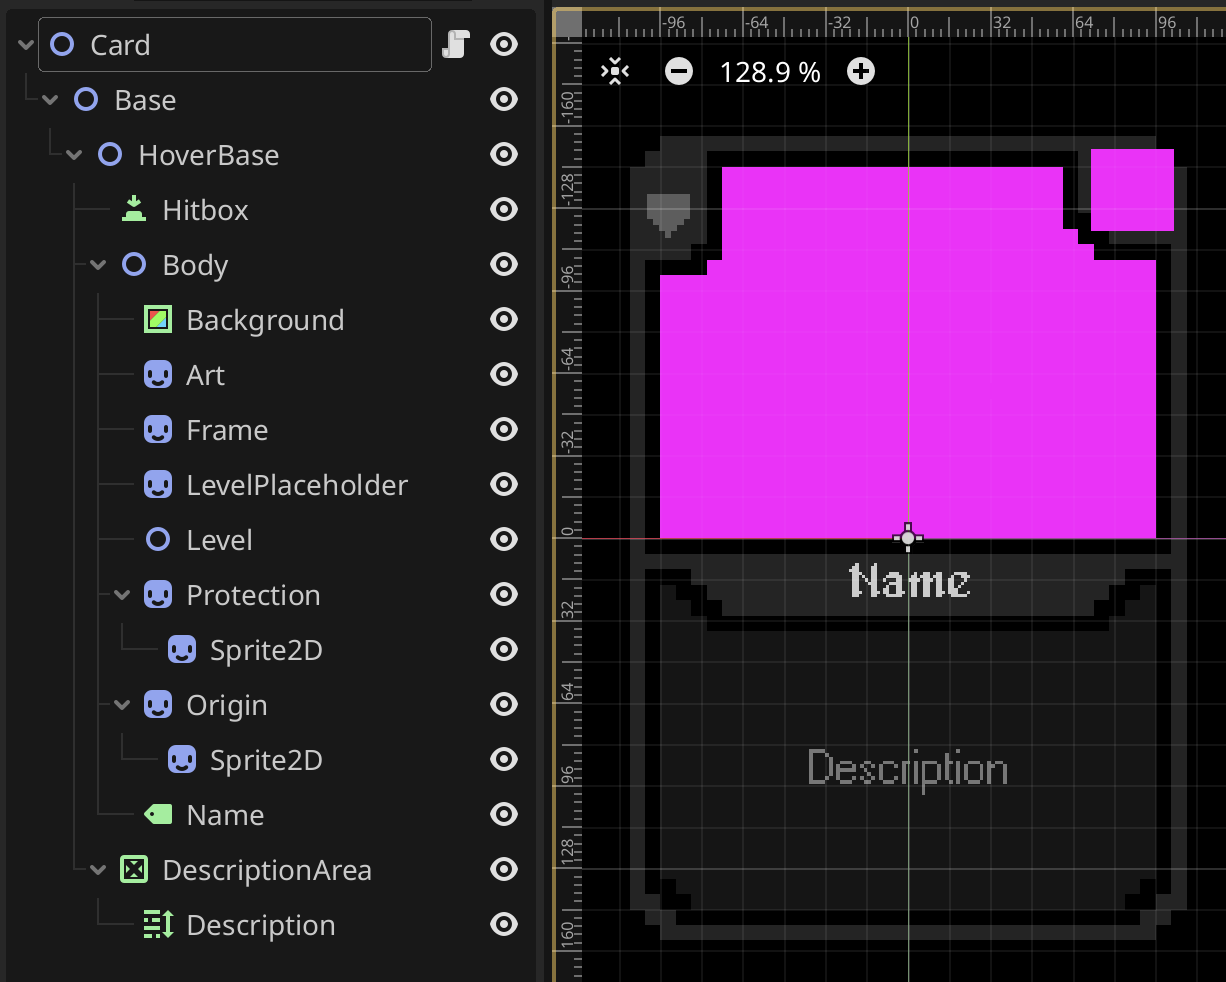
\includegraphics[width=12cm]{images/card_packed_scene.png}
    \caption{The packed scene used for cards}
    \label{figure:card_scene}
\end{figure}

Although enemies do not use packed scenes for it would have required a complete rework of the game's structure, as most game objects, including Enemies, Interactables and the Player, inherit from a base \verb|TileAlignedGameObject| class, which made it complicated to replace enemies with packed scenes. Instead, they are implemented using a script attached to a single \verb|AnimatedSprite2D| node; however, in their \verb|Ready()| method, they add an instance of a \verb|StatusBar| packed scene as a child to themselves. The status bar contains the health and shield bars, plus additional damage, health point, and armor indicators.



\subsection{Turn-based combat}

Initially, the game was intended to be turn-based and would implement a simplified version of the combat system that Baldur's Gate 3\cite{baldursgate2023} uses. This would have meant that enemies would enter a combat state whenever they detect the presence of the player by either noticing them or receiving damage or a status effect from them. Then, based on a defined turn order and each character's own energy points, the player and enemies would take turns in which they can move and use spells, until their energy is depleted. At the beginning of each turn, energy would be replenished. 

An initial version of this system was successfully implemented in an early version of the prototype; however, enemy turns occurred in an instant, without a clear visual representation of each individual action, which made it extremely hard to understand what actually happened between the player's two turns.
To make enemy turns visually appealing and easy-to-follow, I wanted to add small delays between each action they take, for example, they would wait for half a second before every step they take. However, in order not to freeze the whole game while enemy turns last, their animations needed to run on separate threads using asynchronous programming, which added so much unnecessary complexity to the logic of the game, resulting in numerous bugs that were hard to debug due to their multithreaded nature.

Ultimately, for the sake of simplicity, I decided to remove the turn-based combat system in its former state and proceed with a much simpler approach, inspired by the Crypt of the Necrodancer\cite{necrodancer2015}, a 2D top-down rhythm dungeon crawler. Practically, turns got reduced down to a bare minimum: Each player action (movement, interaction, playing, or discarding a card) is considered a whole turn, and thus performing one results in all enemies taking a turn as well. To match the player's reduced flexibility in their turn, the complexity of the enemy logic was also minimized in the same fashion. Although enemies previously had an energy bar that allowed them to take a few steps on their turn, with the new system in place, most of them only step one every other turn.



\subsection{User interface}

\begin{figure}[h]
    \centering
    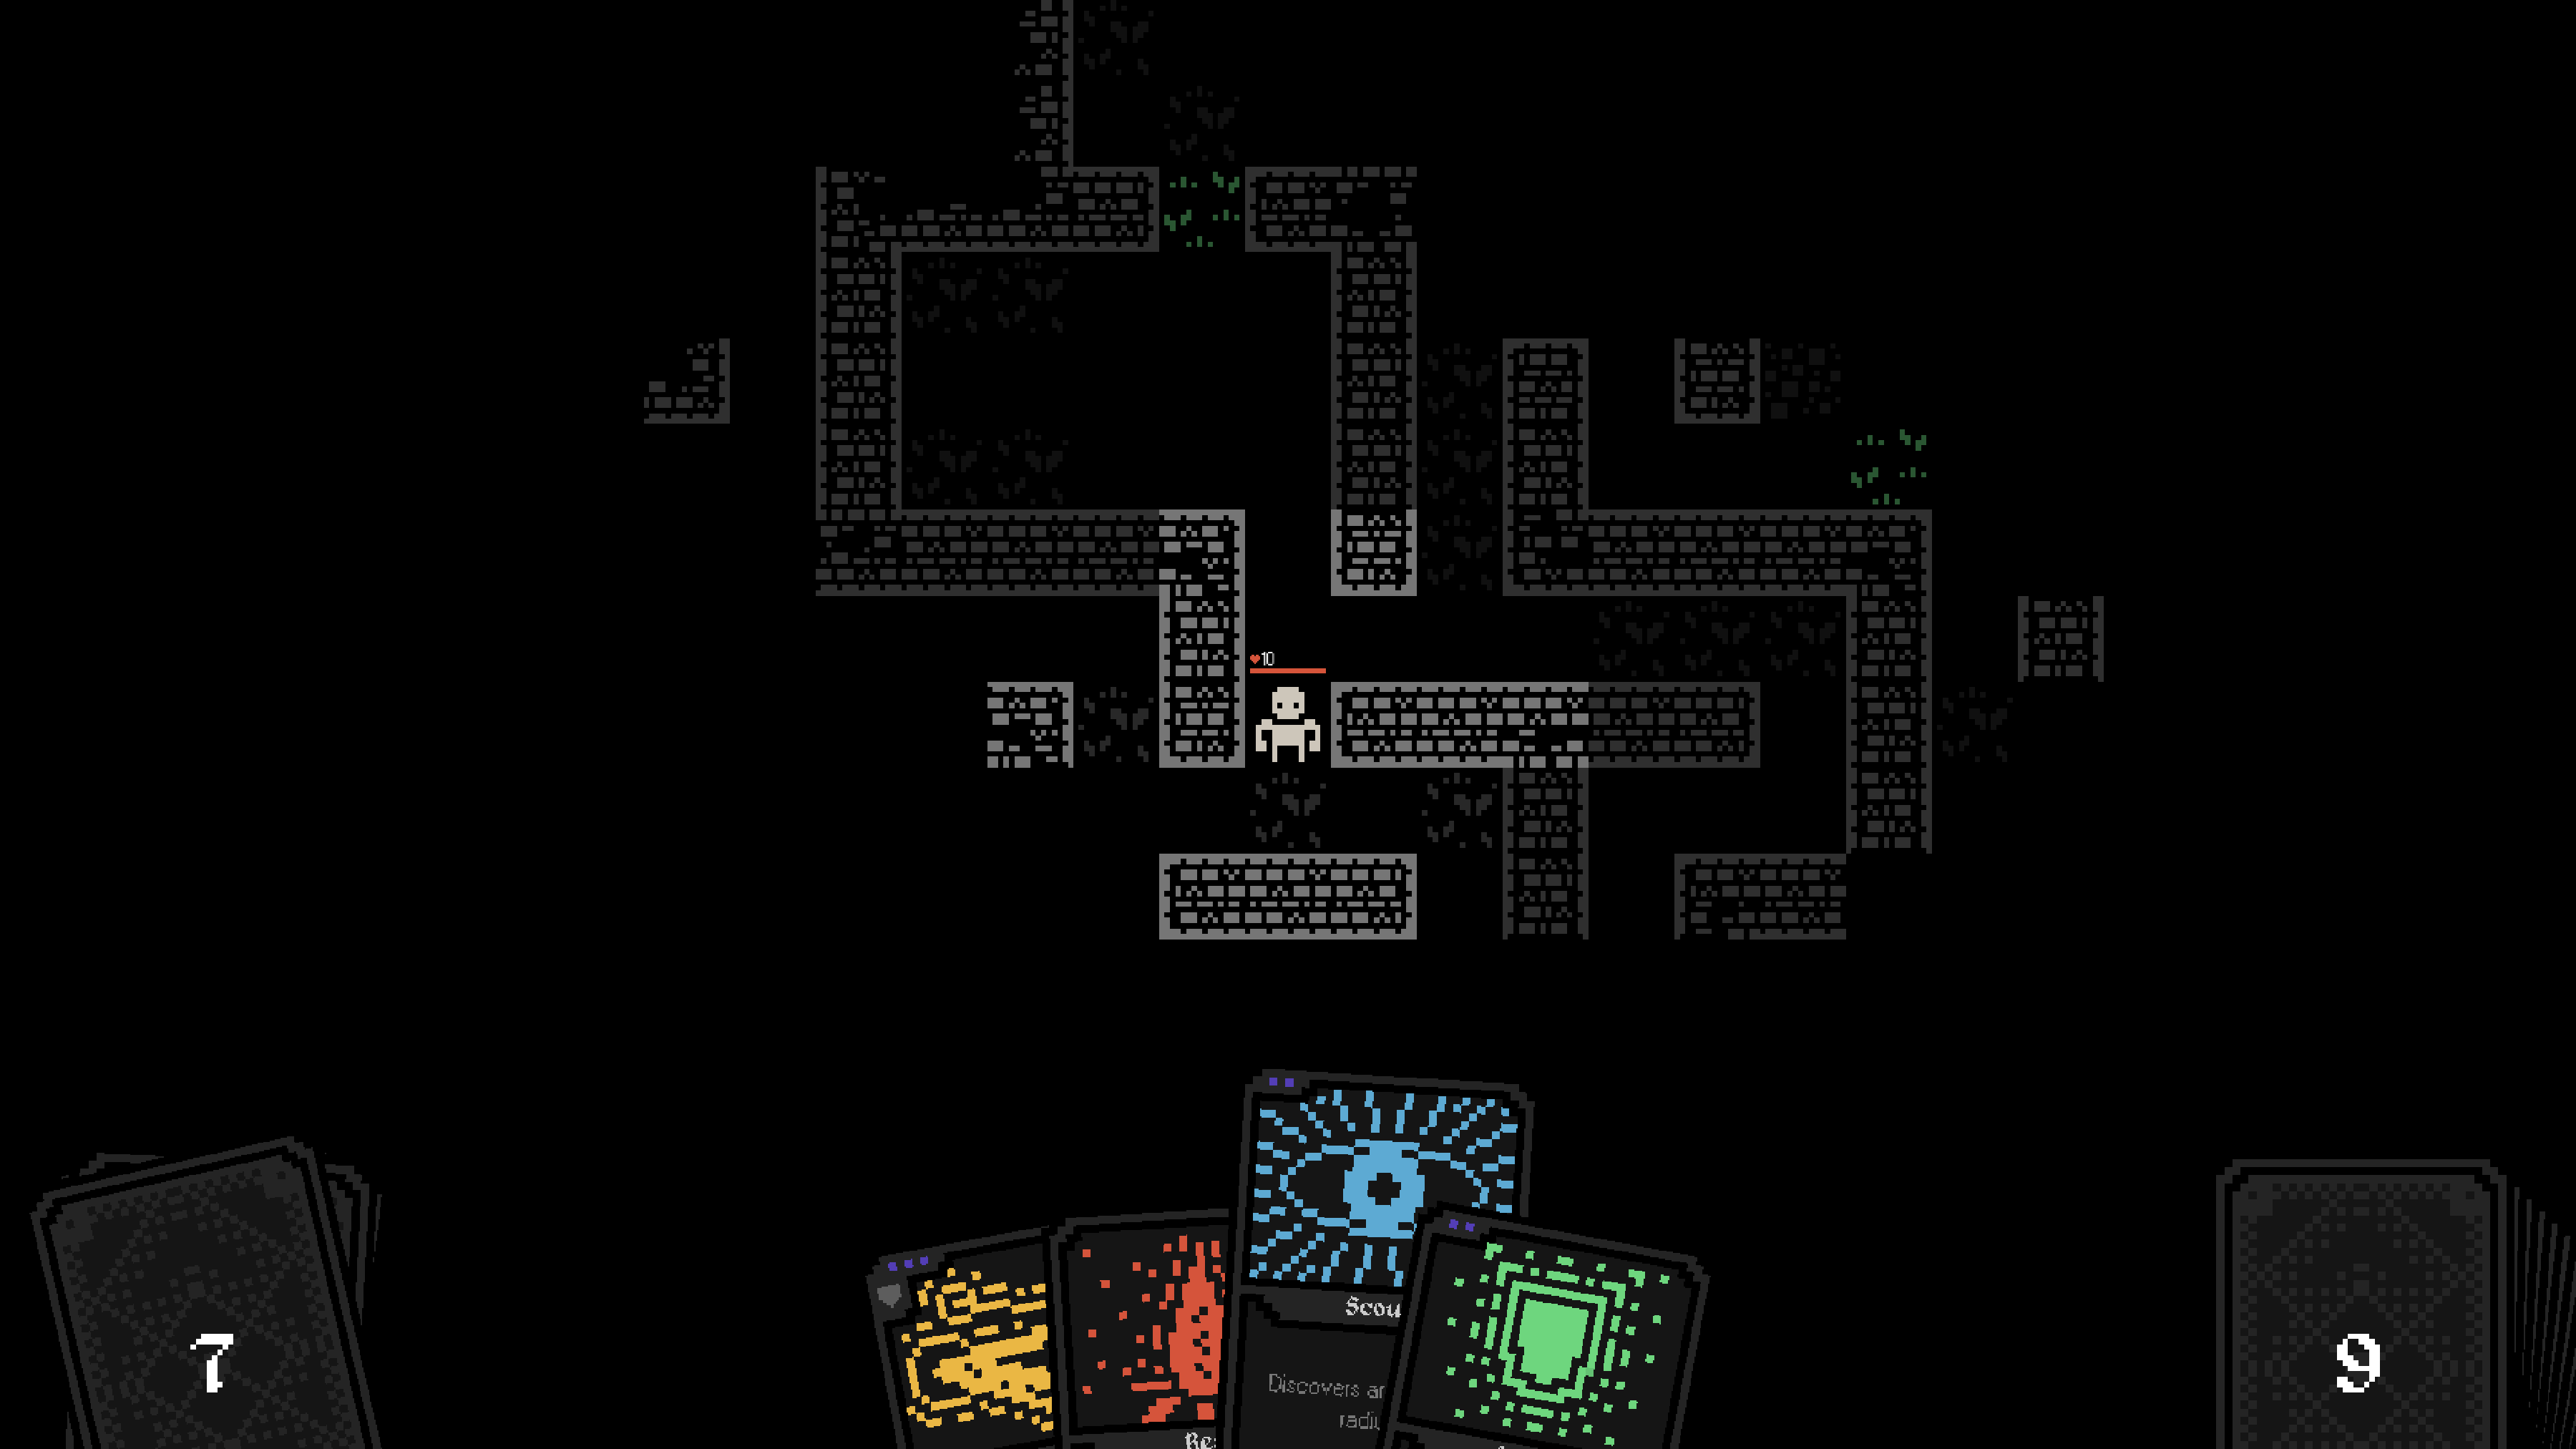
\includegraphics[width=\textwidth]{images/user_interface.png} 
    \caption{The in-game user interface, showing a top-down view of the dungeon, with the discard pile, hand, and deck displayed at the bottom in that order.}
    \label{figure:userInterface}
\end{figure}

The game has a simple user interface during the runs, without much text on it. It has three parts: 

\begin{itemize}
    \item The discard pile, located in the bottom left corner of the screen, where a face-down card is shown with a random orientation for each discarded card. On top of the pile, a number shows the exact number of cards.
    \item The hand in the bottom middle with cards face up, organized in a fan shape, just as someone is holding the cards in their hand. 
    \item The deck in the bottom right corner, which is also a set of face-down cards, but with defined orientations, making it resemble a squared-up pile of cards.
\end{itemize}



\subsection{Controls}

To reduce the scope, the game was designed solely for keyboard and mouse. The movement of the character is controlled with the arrow or the W, A, S, and D keys, as this is standard in any 2D game. For the cards, dragging them with a mouse feels more natural than just selecting one with the arrow keys and then playing it on a key press. Some cards also require the selection of a target, which is also easier to do with a mouse by hovering over and then clicking the target tile, so for these actions there were no alternative controls implemented. The cards can be inspected using a method inspired by Hearthstone\cite{hearthstone2014}: When the player hovers one card in the hand, it slides upward to indicate that it is being hovered (as seen in figure \ref{figure:userInterface}), and to make itself more visible. After the player starts dragging one card, they can end the drag over two areas: the play area covers the upper two-thirds of the screen, and the discard area is located in the bottom left corner.



\subsubsection{Menus}

The game has a pause menu that can be opened by pressing the Escape key. It has four menu items, one for resuming the game, one for quitting it and returning to the desktop, one for opening the help menu, and the last one, which can only be clicked during a run, is for immediately returning to home leaving unprotected cards behind. The help menu includes an explanation of the most important rules of the game and a list of useful tips. Before releasing the game for testing, an additional label was added to the main menu that encourages the tester to open this help menu for further information.

\begin{figure}[h]
    \centering
    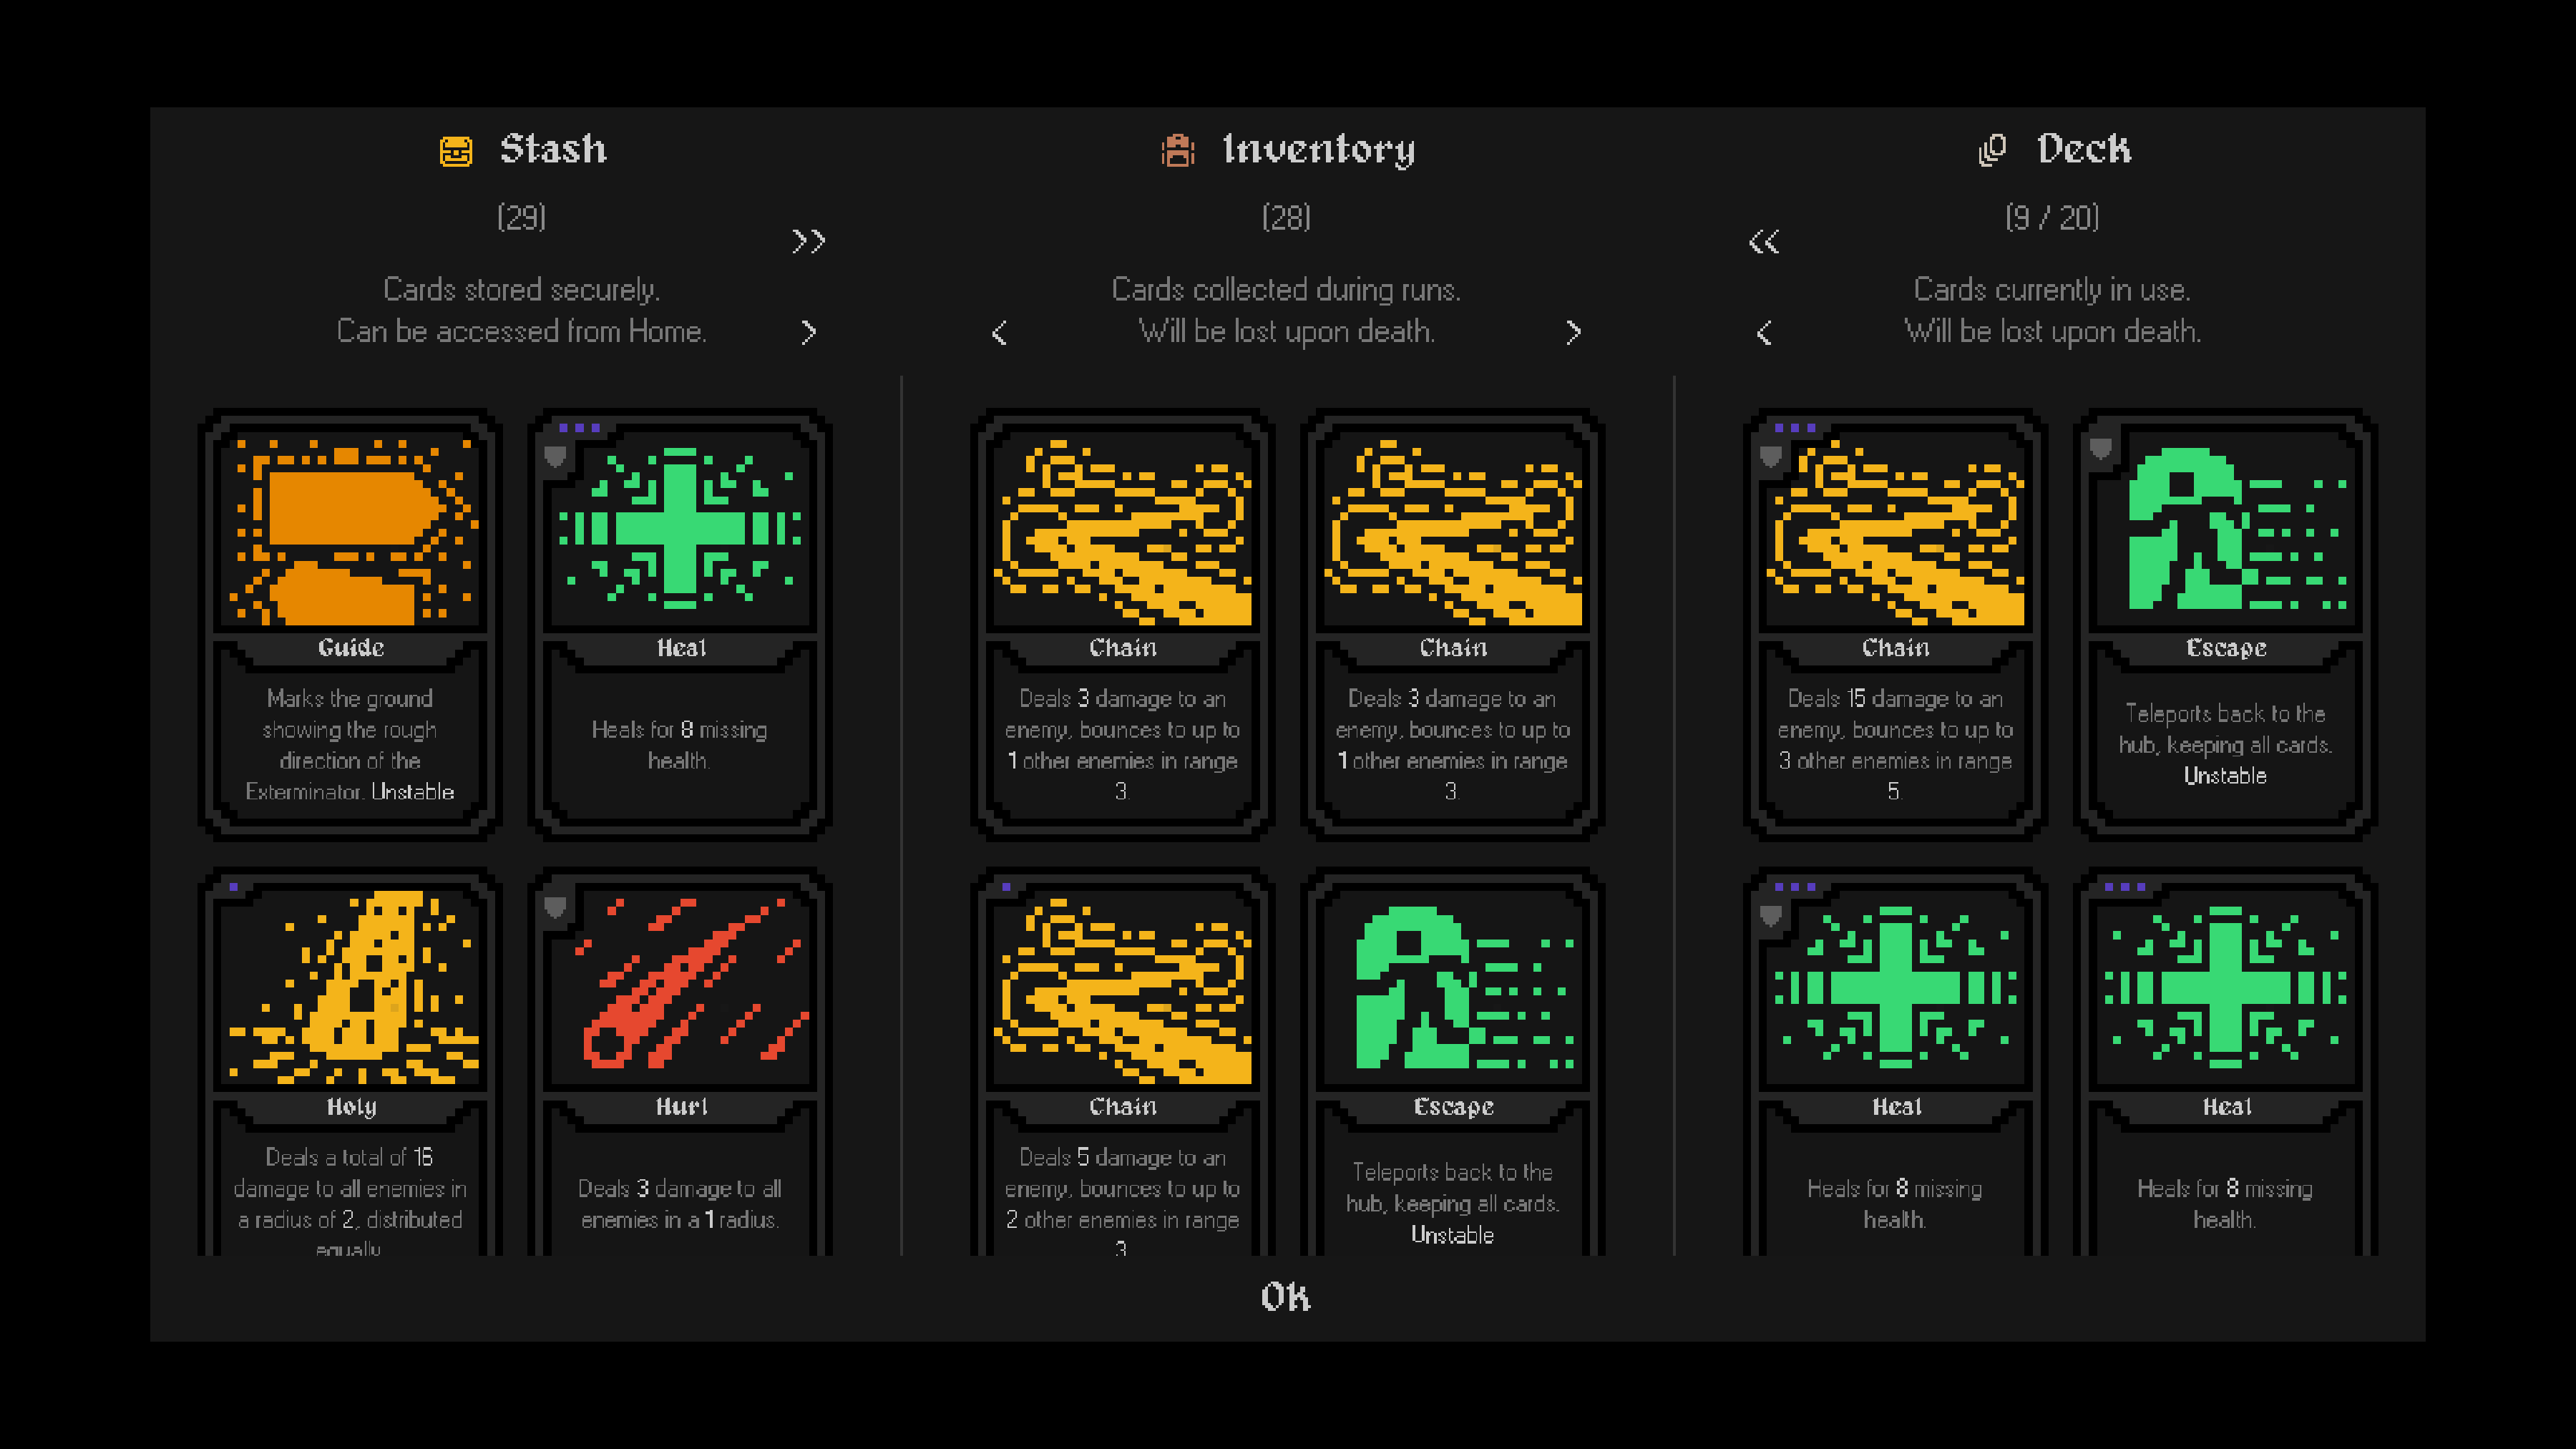
\includegraphics[width=\textwidth]{images/inventory.png} 
    \caption{The inventory menu with three scrollable lists of cards.}
    \label{figure:inventoryMenu}
\end{figure}

In the inventory menu, shown in figure \ref{figure:inventoryMenu}, players are presented with panels containing scrollable sorted lists of cards, one container for cards in the stash, inventory, and deck each. They can move cards between these containers using the mouse, or the arrow buttons located on the top of the panel that allows moving all cards from a container to another one at once.

\begin{figure}[h]
    \centering
    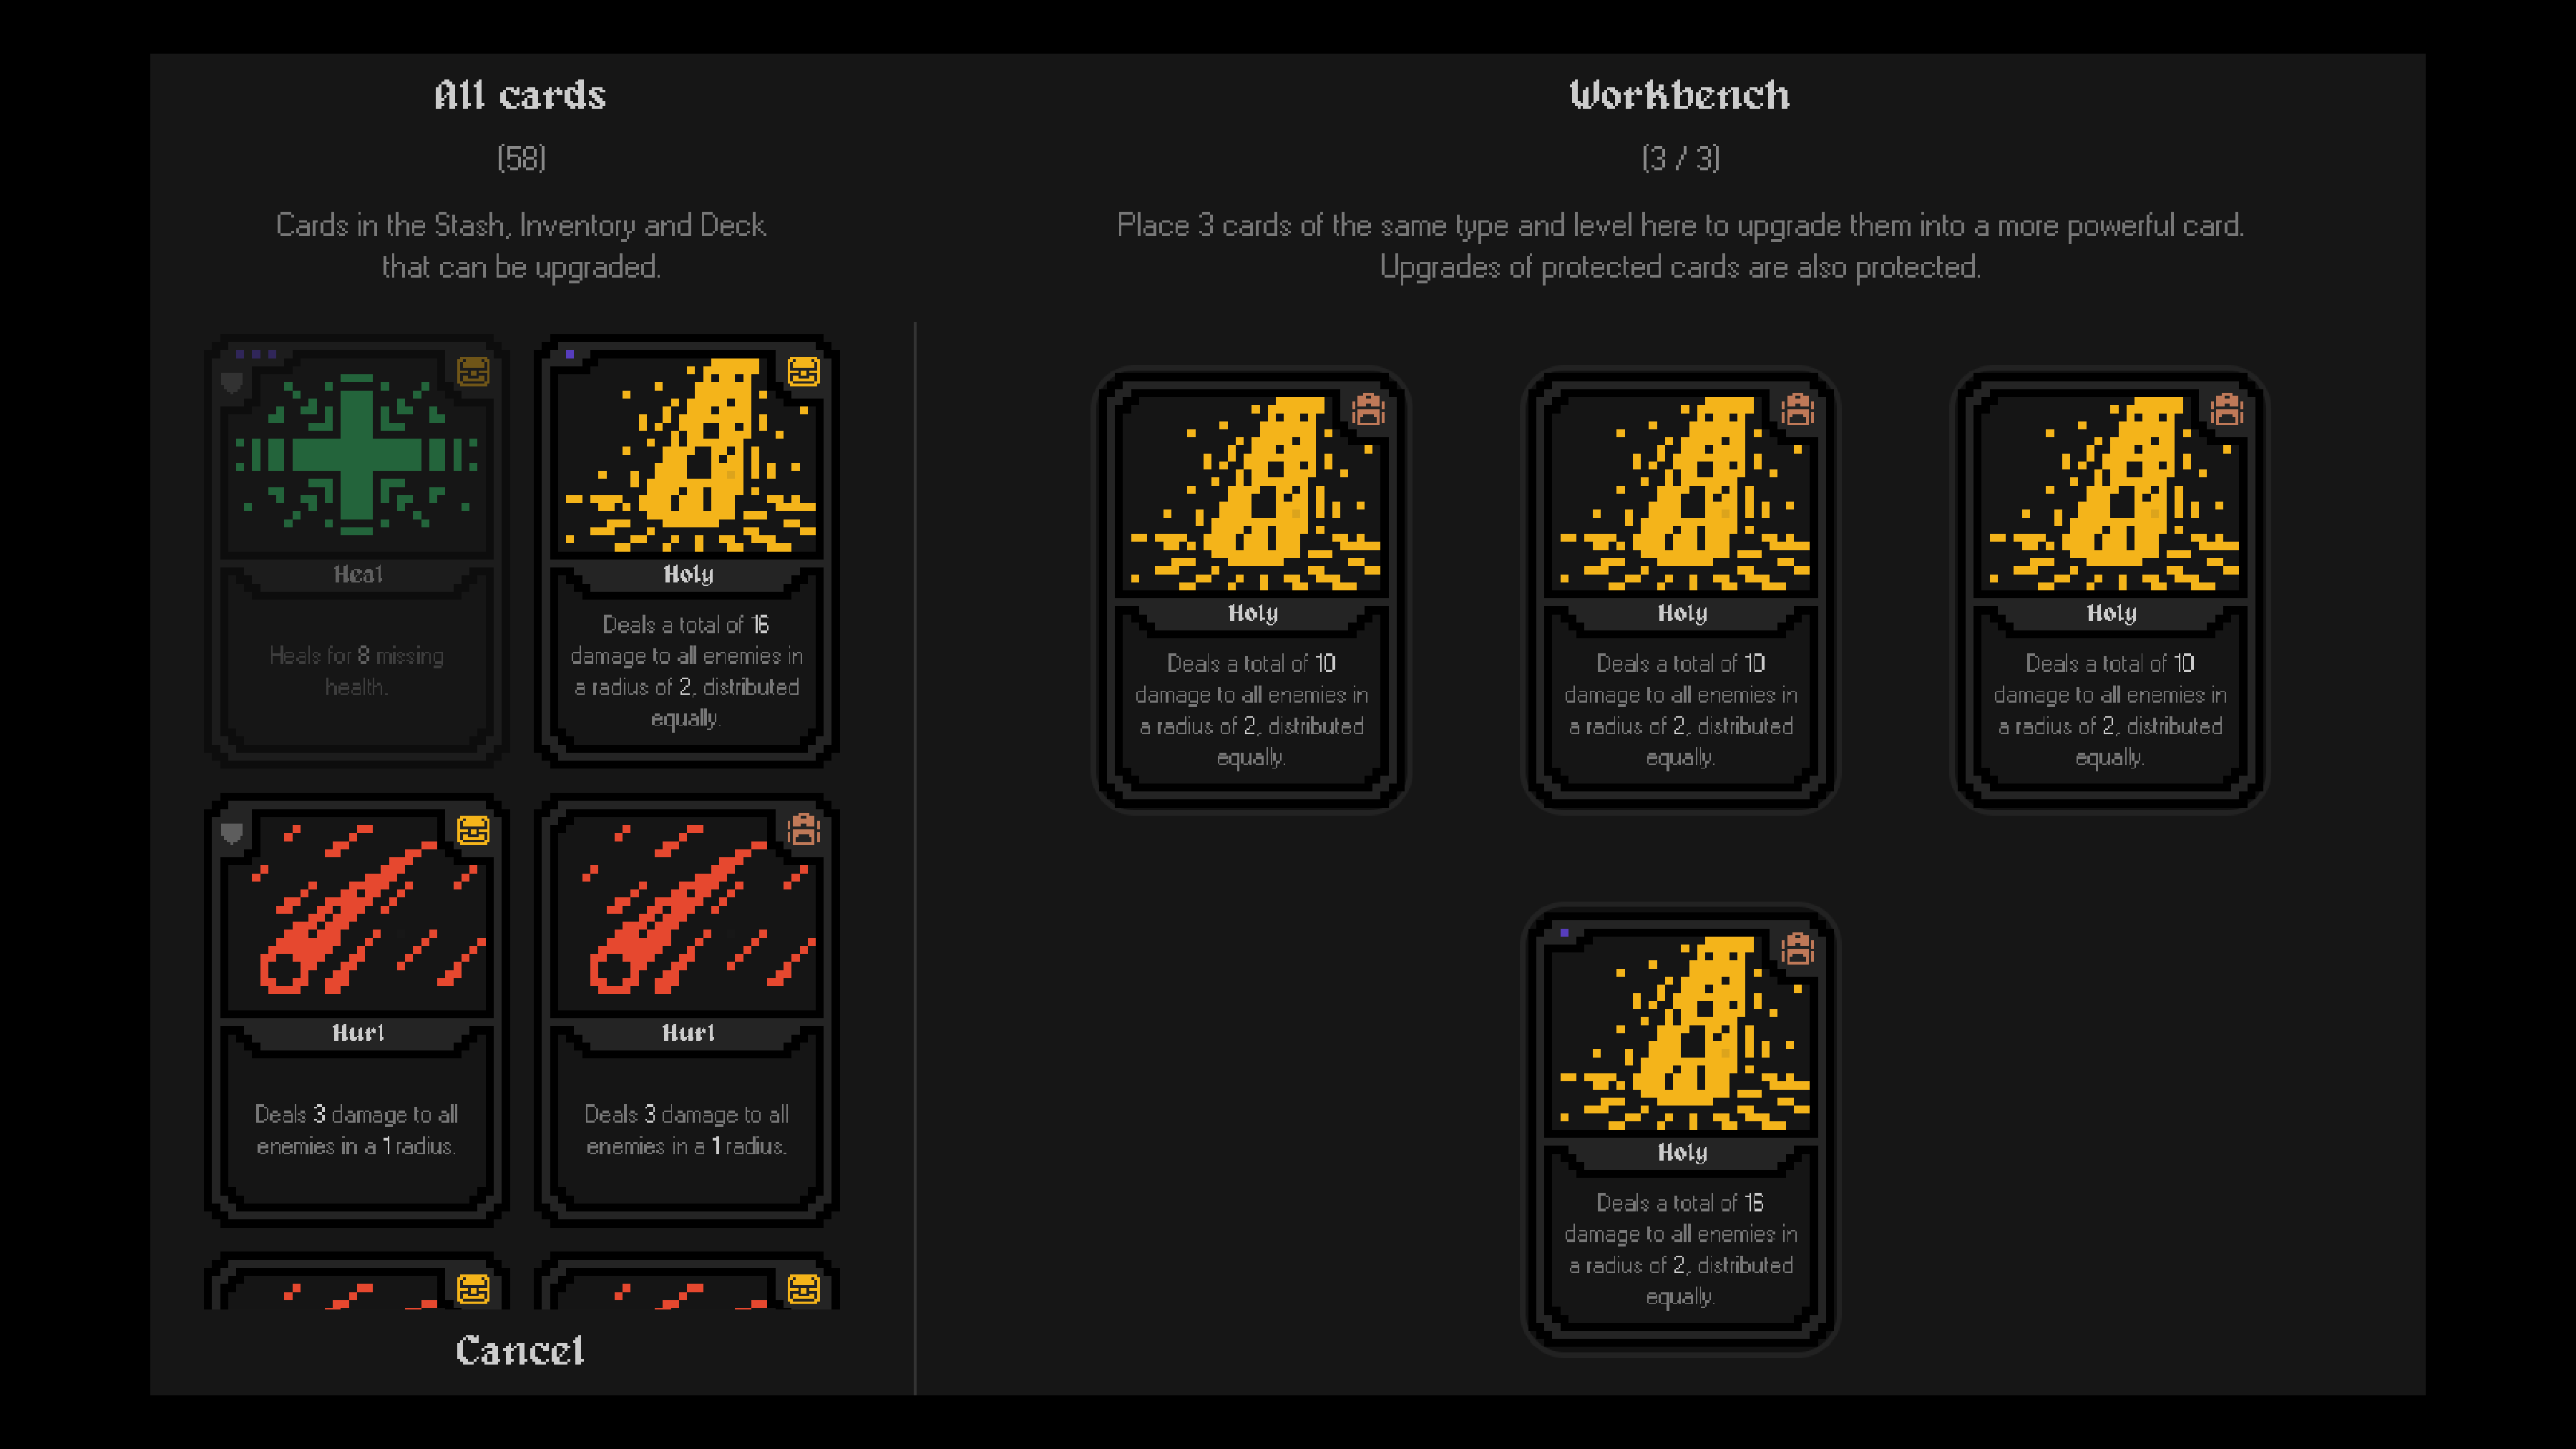
\includegraphics[width=\textwidth]{images/workbench.png} 
    \caption{The workbench menu with a scrollable list of cards, three upgrade slots and one additional slot for the upgraded card.}
    \label{figure:workbenchMenu}
\end{figure}

The workbench, which can be seen in figure \ref{figure:workbenchMenu} also shows a scrollable list of cards on the left side, but this list is a combination of all the cards the player possesses, with each card having an indicator in its upper right corner showing its original location. On the right side, there are one output slot and three input slots in which the player can drag the cards to upgrade them. In this menu, cards can also be clicked to instantly put them into the first available slot or to put them back into the list, making the upgrade process drastically faster.



\subsubsection{Interaction}

The game has several objects with which the player can interact. In early versions, for the interaction to happen, the player had to press a specific key, and then the game checked if the player was standing directly next to any interactable object. If so, then the first of these objects is interacted with. Since the order in which the objects are interacted was not defined, this control method was not straightforward, so it had to be improved.

A method called \textit{nudging} was implemented, which is triggered when the player tries to move into an occupied place, such as a wall or a tile with an enemy or interactable on it. Nudging, just as any other action, also takes one turn, so bumping into walls can even be used to skip turns without moving, allowing enemies to get closer to the player. Nudging an interactable triggers an interaction, and since nudging can only target a single tile, the player has total control over which object they want to interact with.

However, some special objects cannot be interacted with using nudge, as chests, for example, require a key to be opened. Using a \textit{Golden Key} card on a chest instantly opens it, requiring no nudge at all.



\subsubsection{Continuous movement}

Since the dungeon can have long straight corridors, navigating them requires repeatedly pressing the same arrow key many times, which quickly becomes tiring. An alternative movement method was added that allows the player to just hold down an arrow key to keep stepping in that direction at regular intervals. The length of these intervals gradually decreases the longer the key is held down, allowing faster movement while still keeping the turn-based pacing of the game.



\section{Cards}

The most important part of the prototype was to develop a card system with a set of rules. Cards are the only resource in the game, they can be collected during runs and due to the extraction genre, they can also be lost when the player dies, if left unprotected.

In the final design, cards were separated into three containers: the deck contains cards that are in use during a run, the inventory is where the picked up cards go, and the stash is the safe storage where cards remain even after the player dies. Generally, cards cannot be transferred between the three containers, except at home or near a bonfire.

The cards in the deck are divided into three groups, similarly to board games that utilize playing cards.

\begin{enumerate}
  \item \textbf{Hand}: Cards with their face up, that the player is currently holding and is able to play or discard. 
  \item \textbf{Draw pile}: A stack of cards face-down from which the player draws after playing a card from the hand.
  \item \textbf{Discard pile}: Also a stack of cards facing down, where played or discarded cards go.
\end{enumerate}

There is a maximum hand size of 4 and a deck size of 20, and there is no limit on the discard pile. However, the deck size initially was set to 30, which during internal tests felt too much, so it was reduced.



\subsection{Protection}

As mentioned in section \ref{section:concept}, cards can be protected to prevent such edge cases when the player loses all their cards, and thus can no longer do anything in the game. To assist in that and to give the player an opportunity to learn by failing, the starting cards are all protected.

Protection is indicated with a shield symbol in the upper left corner of a protected card. Protection can be carried over to upgraded cards if at least one of the used cards was protected, allowing the player to safely upgrade their starting deck.



\subsection{Single-use cards}

Some cards are considered \textit{utility} cards, most of which can be used once, and then they are lost forever. Such cards are marked with the keyword \textit{Unstable} in their descriptions. These cards, when played, do not go to the discard pile, even when protected; instead, they are lost forever. This feature prevents the exploitation of some powerful cards, such as golden keys, or the later discussed Escape card.



\subsection{Types}

The game in its final state supports four types of cards:

\begin{enumerate}
  \item Targets a single enemy
  \item Targets a single interactable object
  \item targets a location
  \item Targets the player
\end{enumerate}

Except for the cards that target the player, every card is played by first selecting a target tile. Then, based on the tile's content and the card's type, the game determines whether it is a valid target, and then executes the card's ability, or else it cancels the card play.

The game started off with a minimal set of cards: one that heals the player by restoring an amount of missing health points (Heal, type 4), one that damages a single enemy (Smite, type 1), and one that deals damage to all enemies over an area defined by a range (Hurl, type 2). Over time, additional cards were added to enhance the experience and. Some new cards were introduced simply to improve variety, like Holy that damages enemies in an area, similarly to Hurl, but divides the damage equally between all the enemies hit, or Chain that deals damage to a single enemy, like Smite, but then it can jump to another target in range a fixed number of times. Other cards, like Rest and Shuffle were added for balancing reasons.



\subsubsection{Rest}

Rest is a card that shuffles the discard pile into the deck (except for already discarded Rest cards). This allows the player to last significantly longer between bonfire uses or extractions. The introduction of this card was also the main reason the deck size limit was reduced, as putting 15 Rest cards into the deck would allow the player to use the other 15 cards 15 times each (15 x 15 = 225 card uses in total) before needing a bonfire. With a size limit of 20, this mechanic can still be exploited, but the total card uses can only reach a maximum of 100. Additionally, Rest is one of the rarest cards in the game, found only sometimes in chests that require golden key cards, which is also hard to find. So, it is unlikely that the player will ever have 10 Rest cards in their deck.



\subsubsection{Shuffle}

Perhaps the most controversial card based on feedback from internal playtests, as it sometimes felt useless to the testers. It is similar to Rest, except that this time the hand gets shuffled into the deck, and then new cards are drawn. Its intended use is to prevent the player from discarding momentarily undesired cards from the hand, and instead put them away for later use. However, a valid criticism is that the current hand limit, which is four, is too small for this card to play a meaningful role in card management. If the hand capacity were to increase over time, as originally planned, Shuffle would receive more love.



\subsubsection{Guide}

When the final enemy, the Exterminator, was introduced, its location was entirely random, which turned out to be extremely frustrating when the player was actively trying to finish the game by defeating the boss. To resolve this issue, I added an additional, rare utility card called Guide that would mark the ground beneath the player, creating an arrow that points in the approximate direction of the boss, drastically reducing the time spent looking for it. Since this card only becomes useful in the late game, its low drop rate is acceptable early on, as players will likely have acquired at least one by the time they are strong enough to face the boss.



\subsubsection{Teleport}

As the name suggests, this card allows the player to instantly jump to an unoccupied target location. It can be used to bypass closed doors or escape from enemies.



\subsubsection{Shield}

A more powerful alternative to Heal is Shield, which adds extra health points on top of the player's maximum allowed health. When the player receives damage, the shield points are depleted before the health. Shield points have their own bar below the health bar.



\subsubsection{Escape}

The most rare card in the game, Escape allows the player to return home without a ladder, from anywhere. It was only added to have a card that truly feels like a legendary class loot. To prevent it from being too powerful though, it is unstable, so the player cannot reuse it for every run once they find one.



\subsection{Upgrades}

In the original plans, collecting cards was the only meta progression to be included in the prototype. Getting stronger would have been achieved by adding more and more cards to the deck until it is at full capacity, thus the player reaching their full potential. This quickly turned out not to be enough. Getting more and more of the same cards would just mean that the player can repeat the same tasks more during the run without actually feeling stronger.

Card upgrades were implemented as a solution. To upgrade one, three identical cards (the same type and upgrade level) are required at the workbench, a new object that can be found at home. Each card got a maximum upgrade level with predefined values (damage, range, healing amount) depending on level. However, some cards, such as keys and other utility cards, cannot be upgraded as they could not make any significant improvements.



\section{Procedural generation} \label{Section:ProceduralGeneration}

Initially, the game world was meant to be hand-made and quite small. However, I quickly realized that an extraction game needs a large, open map that allows exploration and long run times with sparse extraction points; otherwise, the game might become too easy and repetitive. To accomplish this, hand-crafting the entire map would have been a waste of time, and with fixed extraction point locations, the players could memorize the map and get in and out effortlessly. Instead, I decided to use a procedural dungeon generation algorithm following the method demonstrated by Bob Nystrom\cite{nystromProcedural2014}, extended with the placement of decorations, enemies, and objects. The algorithm consists of six stages:

\begin{enumerate}
  \item First, a number of randomly sized rectangular rooms are placed on the map. If a room overlaps with an already placed one, the new one is discarded. This process is repeated until the predetermined maximum number of attempts is reached.
  \item After the rooms are placed, a random maze generation algorithm is run that carves paths through all the areas that were left empty. As a result, the entire map is now filled with rooms or corridors.
  \item Then hallways are carved out of the walls between the rooms and the maze to make the whole map a single, connected region. Some hallways are generated with a locked door that requires a key to open, somewhat limiting the player's freedom.
  \item Dead ends are removed from the maze to improve exploration. This way every corridor leads to another room and the player will not feel frustrated or misled by paths that go nowhere.
  \item The ground and the walls are decorated based on their surroundings: the adequate wall sprite is selected from a tile map based on its eight neighboring tiles, and the ground is populated with foliage based on its position inside a room or corridor: denser foliage grows along the wall and inside corners.
  \item Finally, rooms are filled with extraction points, bonfires, chests, and enemies based on their size. One exit and one bonfire are always guaranteed, as there are at least two rooms generated exclusively for them. Similarly, a room is reserved for the player to spawn in. With the introduction of the Exterminator, the algorithm was extended with another signature room that is always reserved for the boss.
\end{enumerate}

In later stages of the development, randomized loot generation, along with randomized enemy levels and object density - according to the selected level of difficulty - was also added to the algorithm. With this update, different types of enemies started to drop different loot, defined by a list of probabilities. Additionally, with a higher level of difficulty came more and tougher enemies that yield more loot when defeated; however, extraction points and bonfires became more rare.



\subsection{Pretty walls}

In a tile-based game, walls are usually stored as a two-dimensional array of Boolean variables, where each true value means that the player cannot pass through the corresponding tile. There are multiple ways to illustrate this towards the player, the simplest and probably most boring solution being to use squares of uniform color for each wall tile. Alternatively, walls can be visualized by continuous lines along the connected edges of the wall tiles. However, a more advanced and elegant solution is to create a tile map containing all possible wall shapes and then use the appropriate sprite for each wall tile.

\begin{figure}[h]
    \centering
    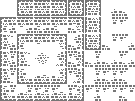
\includegraphics{images/walls.png} 
    \caption{All possible wall textures used in the prototype}
    \label{figure:walls}
\end{figure}

I decided to use a style that, in addition to visualizing the edge, also includes unique details inside the wall, depending on orientation, shape, and width. To achieve this style, there are exactly 48 possible wall shapes and orientations to choose from, shown in figure \ref{figure:walls}.

To retrieve the appropriate sprite from the tile map, I first represented a tile's neighboring eight tiles as a bitmask, the greatest bit storing the value for the top-left neighbor, and following a reading order to store the others, the bottom-right neighbor being the last. Then I create a dictionary object, containing all the possible 256 in total bitmasks as keys, and the atlas coordinates (a two-dimensional vector representing a sprite's position inside the tile set) of their corresponding sprites. To make the process of filling up the dictionary slightly easier, I created patterns (similar to a regular expression or RegEx) consisting of eight nullable booleans, describing the requirements for the bitmasks that correspond to the same sprite in the following way:

\begin{enumerate}
  \item If a bit must be 1 (wall), its value in the pattern is true
  \item If a bit must be 0 (empty), its value in the pattern is false
  \item If it does not matter whether a bit is 1 or 0, its value in the pattern is null
\end{enumerate}

Then the patterns and the atlas coordinates of the desired sprite are passed to a method that generates all possible bitmasks that match the pattern and adds them to the dictionary with the bitmask as the key and the provided coordinate pair as the value.

After the dungeon generation is complete, an additional pass is performed that is responsible for filling the \verb|TileMapLayer| object with the appropriate wall tiles, using the bitmask dictionary.



\subsection{Extraction points}

A defining mechanic of extraction games is the use of extraction points with which players can leave the battlefield and return to a safe zone where they can manage the collected loot and have access to meta-progression systems. In the prototype, ladders were used for such a purpose, which were placed randomly in smaller rooms (specifically in ones sized 3 by 3 or 3 by 5 tiles). If a room was chosen to contain a ladder, enemies were not allowed to be generated inside it.

To exit, players need to approach a ladder and then bump into it (by trying to move onto its occupied tile). As a safety measure, I added a popup text that asks if the player really wants to exit, and to confirm, they are required an extra bump, so that players don't accidentally leave the dungeon.

To exit the dungeon, players must approach a ladder and attempt to move onto its tile (this was called nudging). As a safeguard against accidental exits, a confirmation prompt is triggered on the first interaction. To confirm, the player must bump into the ladder a second time, ensuring they genuinely intend to leave the dungeon.



\subsection{Bonfires}

Bonfires started as a purely aesthetic asset as a reference to the Dark Souls\cite{darksouls2011} series and did not play a role in the gameplay. However, quickly after the development has started, I decided to turn bonfires into an object with which the player can interact by nudging it to heal to maximum health.

After implementing a few cards and the core rules of the game, it became clear that players needed a way to reset their deck by shuffling the discard pile back into it. This would allow for longer runs and potentially justify a lower maximum deck size. The initial solution was to let players trigger a reload manually, similar to reloading a weapon in shooter games, by pressing a button. Like other actions, this took one turn to perform. However, this approach quickly proved to be too powerful, as it placed no meaningful constraints on how often the player could use it. For instance, if a player wanted to draw a specific card, they could simply cycle through the entire deck by repeatedly discarding until the desired card appeared, then reload. Although this cost one action per discard, doing so outside of combat had no real downside, making the mechanic easily abusable.

To limit the usage of reload, the most logical solution appeared to be to tie its use to bonfires, placing them similarly to how ladders were already distributed throughout the map. In addition to reloading the deck, bonfires turned out to also be a perfect mechanic to allow the player to move cards between their deck and inventory, so they could gain access to the cards collected during the run without having to return home.

During internal tests, it was common that multiple bonfires (or ladders, as they were placed the same way) were generated close to each other. Finding such a cluster was a huge advantage, as the player was able to reset their deck multiple times without any need for further exploration; but on the other hand, the rest of the map had a reduced amount of bonfires, which resulted in some runs without finding any. To prevent this, a minimum distance criterion was introduced: if a newly generated bonfire or ladder was too close to any existing one of the same type, it was discarded. This process - similar to the process of how rooms are placed - was repeated until the maximum number of attempts was reached.

When the difficulty parameter was introduced, the minimum distance between bonfires and ladders became tied to it: on higher difficulties, the distance increased, resulting in fewer generated objects and longer exploration sessions.

\todo{Finish + rework with Extraction points section}

